\documentclass{beamer}
\usepackage{graphics}
\usepackage[utf8]{inputenc}
\usepackage{polski}
\usepackage{tikz}
\usepackage{graphicx}

\usetheme{Bergen}

\begin{document}
\title{Optical Character Recognition}
\author{Gleb Peregud}

\frame{\titlepage}

\frame
{
  \frametitle{What is OCR?}
  It is the mechanical or electronic translation of scanned images of
  handwritten, typewritten or printed text into machine-encoded text.
}

\frame{
  \frametitle{History}
  \begin{itemize}
  \item 1929 Gustav Tauschek, Germany, first patent. Templates and photodetector
  \item 1950 David H. Shepard, USA, Army Forces Security
    Agency. Intelligent Machines Research Corporation
  \item 1955 Readers Digest. First commercial system
  \item 1965 US Postal Service. Sort mail
  \item 1965 UK General Post Office. Sort mail
  \item 1974 Ray Kurzwell. Omni-font optical OCR. For blind
  \end{itemize}
}

\frame{
  \frametitle{Parts of the problem}
  \begin{itemize}
  \item Character recognition
  \item Word recognition
  \item Grammar analysis
  \item Image detection
  \item Page layout recognition
  \item Recreation of original page
  \end{itemize}
}

\frame{
  \frametitle{Character recognition}
  \begin{block}{What?}
  Classifying image samples into defined set of classes,
  corresponding to characters available in a given script.
  \end{block}
}

\frame{
  \frametitle{Problems}
  \begin{itemize}
  \item Scripts
  \item Fonts
  \item Distortions
    \begin{itemize}
    \item skew
    \item noise
    \item occlusions
    \item rotation
    \end{itemize}
  \item Handwriting style
  \end{itemize}
}

\frame{
  \frametitle{Preparations}
  \begin{itemize}
  \item Scanning
  \item Binarization or greyscaling
  \item Character separation
  \item Deskewing
  \item Noise removal
  \item Occlusion removal
  \item Blurring
  \item Centering
  \item Normalization
  \end{itemize}
}

\frame{
  \frametitle{Approaches}
  \begin{itemize}
  \item ANN
    \begin{itemize}
    \item linear classifier
    \item multilayer NN
    \item convolution nets
    \end{itemize}
  \item SVM
  \item Decision trees
    \begin{itemize}
    \item stumps
    \item Haar features
    \end{itemize}
  \item Other
    \begin{itemize}
    \item Contour-based (contour matching, direction codes)
    \item Feature extraction
    \item Contour matching
    \item Histograms
    \end{itemize}
  \end{itemize}
}

\frame{
  \frametitle{Invariants}
  \begin{itemize}
    \item augment training set with modified samples transformed with
      invariants
    \item build in invariances by extracting invariant features
    \item add regularization term to error function
    \item change structure of classifier to ensure invariance
  \end{itemize}
}

\frame{
  \frametitle{MNIST database}
  \begin{block}{Name}
    THE MNIST DATABASE of handwritten digits
  \end{block}
  \begin{block}{Who}
    Yann LeCun, Courant Institute, NYU \\
    Corinna Cortes, Google Labs, New York
  \end{block}
  \begin{itemize}
    \item 28x28 images
    \item centered by center of mass
    \item gray-scale
    \item 60000 training set
    \item 10000 test set
  \end{itemize}
}

\frame{
  \frametitle{Neural networks 0}
  \begin{block}{Who?}
    Gleb Peregud, 2011
  \end{block}
  \begin{block}{What?}
    \begin{itemize}
    \item 2-layer NN
    \item 784-10
    \item quickprop
    \end{itemize}
  \end{block}
  \begin{block}{Result}
    15\%
  \end{block}
}

\frame{
  \frametitle{Neural networks 1}
  \begin{block}{Who?}
    LeCun et al. 1998
  \end{block}
  \begin{block}{What?}
    \begin{itemize}
    \item 3-layer NN
    \item 784-1000-10
    \item no preparations
    \end{itemize}
  \end{block}
  \begin{block}{Result}
    4.5\%
  \end{block}
}

\frame{
  \frametitle{Neural networks 2}
  \begin{block}{Who?}
    Ciresan et al., arXiv 1003.0358, 2010
  \end{block}
  \begin{block}{What?}
    \begin{itemize}
    \item 7-layer NN
    \item 784-2500-2000-1500-1000-500-10
    \item trained on GPU
    \item additional training with elastic distortions
    \end{itemize}
  \end{block}
  \begin{block}{Result}
    0.35\%
  \end{block}
}

\frame{
  \frametitle{Convolution networks}
  \begin{itemize}
  \item special neural network where only pixel values around a
    central pixels go into the network’s hidden units (sparse
    network) and they share their weights
  \item network performs a nonlinear filtering operation
  \item do subsampling - the outputs of the hidden units go into a
    smaller set of hidden units
  \item optional - repeat until a normal output layer
  \item contain less parameters than full networks, and are therefore easier to train
  \item their structure is modeled on the human visual system
  \end{itemize}
}

\frame{
  \frametitle{Convolution networks - example}
  \begin{block}{Who?}
    LeCun et al. 1998
  \end{block}
  \begin{block}{What?}
    \begin{itemize}
    \item convolutional network LeNet-5
    \item trained with distortions
    \item works with little-to-no image preprocessing
    \item works directly on RGB images
    \item can recognize patterns with extreme variability
    \end{itemize}
  \end{block}
}

\frame{
  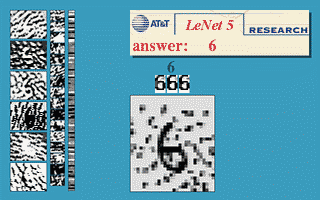
\includegraphics[width=23em]{noise6.png}
}

\frame{
  \frametitle{K-NN, contour matching using shape contexts}
  \begin{block}{Who?}
    Belongie et al. IEEE PAMI 2002
  \end{block}
  \begin{block}{What?}
    \begin{itemize}
    \item contour detection
    \item shape context calculation
    \item contour point matching
    \item iterative transformations (TPS, affine)
    \item selecting of prototypes
    \item K-NN for classification
    \end{itemize}
  \end{block}
  \begin{block}{Result}
    0.63\%
  \end{block}
}

\frame{
  
\includegraphics[width=25em]{two-digits.png}
}

\frame{
  \frametitle{Shape context}
  \begin{block}{What?}
    Histogram in log-polar space
  \end{block}
  \begin{itemize}
  \item counts number of points in each bin relative to a selected
    point
  \item compact and rich local descriptor
  \item similar points on a contour have similar shape contexts
  \item similarity in terms of $\chi^{2}$
  \end{itemize}
}

\frame{
  \frametitle{Shape context}
  
\includegraphics[width=23em]{shape-contexts.png}
}

\frame{
  \frametitle{Shape context matching cost}
  \[ C_{ij} = (1 - \beta)C_{ij}^{sc} + \beta{}C_{ij}^{tan} \]
  \\
  \[ C_{ij}^{tan} = 0.5(1 - cos(\theta_{i} - \theta_{j})) \]

}

\frame{
  \frametitle{Matching points on contours}
  \begin{itemize}
  \item Hungarian algorithm
  \item minimizes \[ H(\pi) = \sum_{i} C(p_i,q_{\pi(i)}) \]
  \item $O(n^3)$
  \end{itemize}
}

\frame{
  \frametitle{Shape context, transformations}
  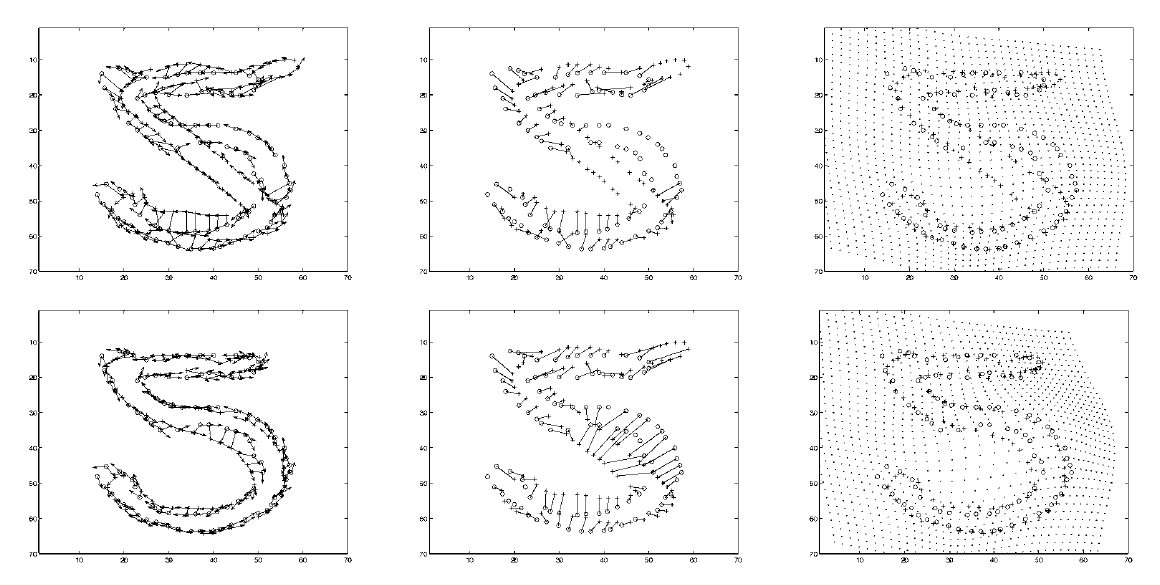
\includegraphics[width=23em]{process.png}
}

\frame{
  \frametitle{Shapes similarity distance}
  \begin{itemize}
  \item \[ D = 1.6D_{ac} + D_{sc} + 0.3D_{be} \]
  \item $D_{ac}$ is defined as the sum of squared brightness
    differences in Gaussian windows around corresponding image points
  \item $D_{sc}$ is defined as as the symmetric sum of shape context matching
    costs over best matching points
  \item $D_{be}$ is a bending energy of TPS transformation
  \end{itemize}
}

\frame{
  \frametitle{Classifier}
  \begin{itemize}
  \item select k prototypes for each digit
  \item use PAM / k-medoids algorithm
  \item run k-nearest neighbours algorithm for input on prototypes
  \end{itemize}
}

\frame{
  Thank you!
}

% \frame{
%   \frametitle{Pożądane właściwości}
%   \begin{itemize}
%   \item działa w chmurze
%   \item minimalne wymagania konfiguracyjne
%   \item łatwe w użyciu
%   \item nieinwazyjne
%   \item rozszerzalne
%   \item działa :)
%   \end{itemize}
% }

% \frame{
%   \frametitle{Stosowane technologie}
%   \parbox{.4\textwidth}
%   % {\hspace{2em}\includegraphics[width=.3\textwidth]{erlang_logo.png}}
%   \parbox{.5\textwidth}
%   {
%   \begin{itemize}
%     \item Erlang
%     \pause
%     \item eXAT
%     \pause
%     \item ERESYE
%     \pause
%     \item Folsom
%     \pause
%     \item inet-mdns
%   \end{itemize}
%   }
% }

% \frame{
%    \frametitle{Rodzaje agentów}
%    Agent monitorujący
%    \begin{itemize}
%    \item działa na każdym węźle chmury
%    \item odpowiedzialny za całą logikę systemu
%      \begin{itemize}
%        \item zbieranie informacji o otoczeniu
%        \item użycie regułek do wnioskowania w celu uzupełniania
%          posiadanych informacji
%      \end{itemize}
%    \end{itemize}
%    \pause
%    Agent administratora
%    \begin{itemize}
%    \item uruchamiany przez administratora
%    \item pobiera dane do raportu od agentów monitorujących
%    \item prezentuje raport w~czytelnej formie
%      \begin{itemize}
%      \item wnioskowanie na podstawie zebranej wiedzy
%      \end{itemize}
%    \end{itemize}
%    }

% \frame{
%    \frametitle{Dane posiadane przez agenta}
%    \begin{itemize}
%    \item nazwa własna
%    \item uługi świadczone przez dany węzeł
%    \item procesy powiązane z~usługami
%      \begin{itemize}
%      \item sposoby wykrycia czy proces jest uruchomiony (np. regex)
%      \end{itemize}
%    \item lista wszystkich znanych węzłów chmury
%    \item lista sąsiadów (obserwowanych węzłów)
%    \item liczba agentów obserwujących węzeł
%    \end{itemize}
% }

% % \frame{
% %    \frametitle{Dane posiadane przez agenta}
% %    \begin{center}
% %    \begin{tikzpicture}[every node/.style={circle,draw}]
% %    \node[xshift=-5em,yshift=2em] (a) {1};
% %    \node (b) {1};
% %    \node[xshift=5em,yshift=1em] (c) {2};
% %    \node[xshift=2em,yshift=-6em] (d) {2};
% %    \node[xshift=-2em,yshift=-5em] (e) {2};
% %    \node[xshift=8em,yshift=-3em] (f) {2};
% %    \draw[-latex] (a) -- (b);
% %    \draw[-latex] (b) -- (c);
% %    \draw[-latex] (c) -- (d);
% %    \draw[-latex] (d) -- (e);
% %    \draw[-latex] (e) -- (f);
% %    \draw[-latex] (a) -- (e);
% %    \draw[-latex] (a) -- (c);
% %    \draw[-latex] (c) -- (f);
% %    \draw[-latex] (b) -- (d);
% %    \draw[-latex] (e) .. controls +(-2em,1em) and +(-1em,-2em) .. (a);
% %    \end{tikzpicture}\\[.5em]
% %    Obserwujący i~obserwatorzy
% %    \end{center}
% %    }

% \frame{
%    \frametitle{Dane posiadane przez agenta}
%    \begin{overlayarea}{\textwidth}{.5\textheight}
%    \only<1>{
%       Dla małych klastrów:\\[1em]
%       \hspace{1.5em}lista sąsiadów $=$ lista wszystkich węzłów
%    }
%    \only<2->{
%       Dla dużych klastrów:\\[1em]
%       \hspace{1.5em}Listy sąsiadów generowane dynamicznie.\\[1em]
%       \only<3>{\hspace{3em}\parbox{0.8\textwidth}{Stosowany popularny algorytm
%       równoważenia obciążeń (np. dyfuzja naturalna).}}
%    }
%    \end{overlayarea}
% }

% \frame{
%    \frametitle{Zbieranie danych}
%    \begin{enumerate}
%    \item agent otrzymuje żądanie przesłania danych
%    \pause
%    \item sprawdza, czy pobrał dane od sąsiadów w~ostatnim czasie
%    \pause
%    \item wysyła żądania do sąsiadów, których dane są nieaktualne
%    \pause
%    \item jeśli dostanie wielokrotnie dane tego samego węzła, wybiera aktualniejsze
%    \pause
%    \item dodaje do listy własne dane
%    \pause
%    \item wysyła odpowiedź
%    \end{enumerate}
%    \pause
%    Węzły, które zostały już odpytane na wyższym poziomie, są pomijane
%    (unikanie cykli).
% }

% \frame{
%    \frametitle{Sposób komunikacji}
%    Mechanizm komunikacji eXATa:
%    \pause
%    \begin{itemize}
%    \item zgodny z~FIPA ACL
%    \pause
%    \item oparty na protokole HTTP MTP
%    \pause
%    \item<alert@5>wymaga nazwy agenta i~adresu sieciowego
%    \end{itemize}
%    }

% \frame{
%    \frametitle{Sposób komunikacji}
%    Agenci wykrywają się automatycznie\\[1em]
%    \pause
%    \hspace{1.5em}W~sieci LAN: mDNS (Zeroconf)\\[.5em]
%    \pause
%    \hspace{1.5em}W~Amazon EC2 (i~innych): import listy węzłów z API EC2
%    }

% \frame{
%    \frametitle{Rodzaje komunikatów}
%    \only<1>{
%       \textbf{agent-ping}\\[1em]
%       \hspace*{.05\textwidth}\parbox{0.95\textwidth}{
%       Typ ACL: \emph{request}\\[.5em]
%       Dodatkowe dane: brak\\[.5em]
%       Komunikat kontrolny warstwy agentów}
%       }
%    \only<2>{
%       \textbf{agent-pong}\\[1em]
%       \hspace*{.05\textwidth}\parbox{0.95\textwidth}{
%       Typ ACL: \emph{inform}\\[.5em]
%       Dodatkowe dane: brak\\[.5em]
%       Komunikat kontrolny warstwy agentów}
%       }
%    \only<3>{
%       \textbf{ping-other}\\[1em]
%       \hspace*{.05\textwidth}\parbox{0.95\textwidth}{
%       Typ ACL: \emph{request}\\[.5em]
%       Dodatkowe dane: adres docelowego węzła\\[.5em]
%       Komunikat kontrolny przekierowywany przez trzeciego agenta}
%       }
%    \only<4>{
%       \textbf{pong-other}\\[1em]
%       \hspace*{.05\textwidth}\parbox{0.95\textwidth}{
%       Typ ACL: \emph{inform if}\\[.5em]
%       Dodatkowe dane: adres odpowiadającego węzła\\[.5em]
%       Komunikat kontrolny przekierowywany przez trzeciego agenta}
%       }
%    \only<5>{
%       \textbf{request-metrics}\\[1em]
%       \hspace*{.05\textwidth}\parbox{0.95\textwidth}{
%       Typ ACL: \emph{request}\\[.5em]
%       Dodatkowe dane: lista węzłów już odpytywanych\\[.5em]
%       Żądanie przesłania danych wydajnościowych}
%       }
%    \only<6>{
%       \textbf{metrics-list}\\[1em]
%       \hspace*{.05\textwidth}\parbox{0.95\textwidth}{
%       Typ ACL: \emph{inform}\\[.5em]
%       Dodatkowe dane: pary agentów i~danych wydajnościowych\\[.5em]
%       Przesłane dane wydajnościowe}
%       }
%    \only<7>{
%       \textbf{request-services}\\[1em]
%       \hspace*{.05\textwidth}\parbox{0.95\textwidth}{
%       Typ ACL: \emph{request}\\[.5em]
%       Dodatkowe dane: lista węzłów już odpytywanych\\[.5em]
%       Żądanie przesłania danych wydajnościowych}
%       }
%    \only<8>{
%       \textbf{services-list}\\[1em]
%       \hspace*{.05\textwidth}\parbox{0.95\textwidth}{
%       Typ ACL: \emph{inform}\\[.5em]
%       Dodatkowe dane: pary agentów i~świadczonych przez nie usług\\[.5em]
%       Przesłane dane o~usługach}
%       }
% }

% \frame{
%    \frametitle{Wykrywane scenariusze}
%    \only<1>{
%       Nie działający agent
%       \begin{itemize}
%       \item brak odpowiedzi na \textbf{agent-ping}
%       \item normalna odpowiedź na ping w~warstwie sieciowej
%       \end{itemize}
%       }
%    \only<2>{
%       Nie działający węzeł
%       \begin{itemize}
%       \item brak odpowiedzi na \textbf{agent-ping}
%       \item brak odpowiedzi na ping w~warstwie sieciowej
%       \item brak odpowiedzi na pingi przekierowywane przez sąsiadów
%       (\textbf{ping-other})
%       \end{itemize}
%       }
%    \only<3>{
%       Przerwane łącze
%       \begin{itemize}
%       \item brak odpowiedzi na \textbf{agent-ping}
%       \item brak odpowiedzi na ping w~warstwie sieciowej
%       \item normalna odpowiedź na pingi przekierowywane przez sąsiadów
%       (\textbf{ping-other})
%       \end{itemize}
%       }
%    \only<4>{
%       Zagrożona usługa
%       \begin{itemize}
%       \item świadczące ją węzły nie działają\\[.5ex]
%       \hspace{1em}lub\\
%       \item świadczące ją węzły są przeciążone\\[.5ex]
%       \hspace{1em}lub\\
%       \item procesy związane z~usługą zabite
%       \end{itemize}
%       }
%    }

% \frame{
%    \frametitle{Potencjalne problemy projektu}
%    \begin{itemize}
%    \item trudności z~wykorzystywanymi bibliotekami
%    \pause
%    \item problemy z~konfiguracją środowiska testowego
%    \pause
%    \item za duże użycie zasobów sieciowych
%    \pause
%    \item wdrożenie systemu (patrz p.1)
%    \pause
%    \item mała ilość czasu
%    \end{itemize}
%    }

% % \frame{
% %   \includegraphics[width=\textwidth]{clouds.jpg}
% %    }

\end{document}

